\subsection{Klassediagram og metodebeskrivelse}
Ud fra implementeringen er der genereret illustrerende klassediagrammer som kan ses på figur \ref{fig:GUI_KD}, disse klasser ligger under Libary, som kan ses på figur \ref{fig:web}, klasserne er anvendt til at kunne oprette objekter, både ud fra indholdet i databasen og til at lave en Socket klient. Hvis der ønskes yderligere indsigt i hvordan specifik kode er skrevet henvises der til sourcekoden\footnote{Se bilag under Software\textbackslash www\textbackslash lib}.

\begin{figure}[H]
    \centering
    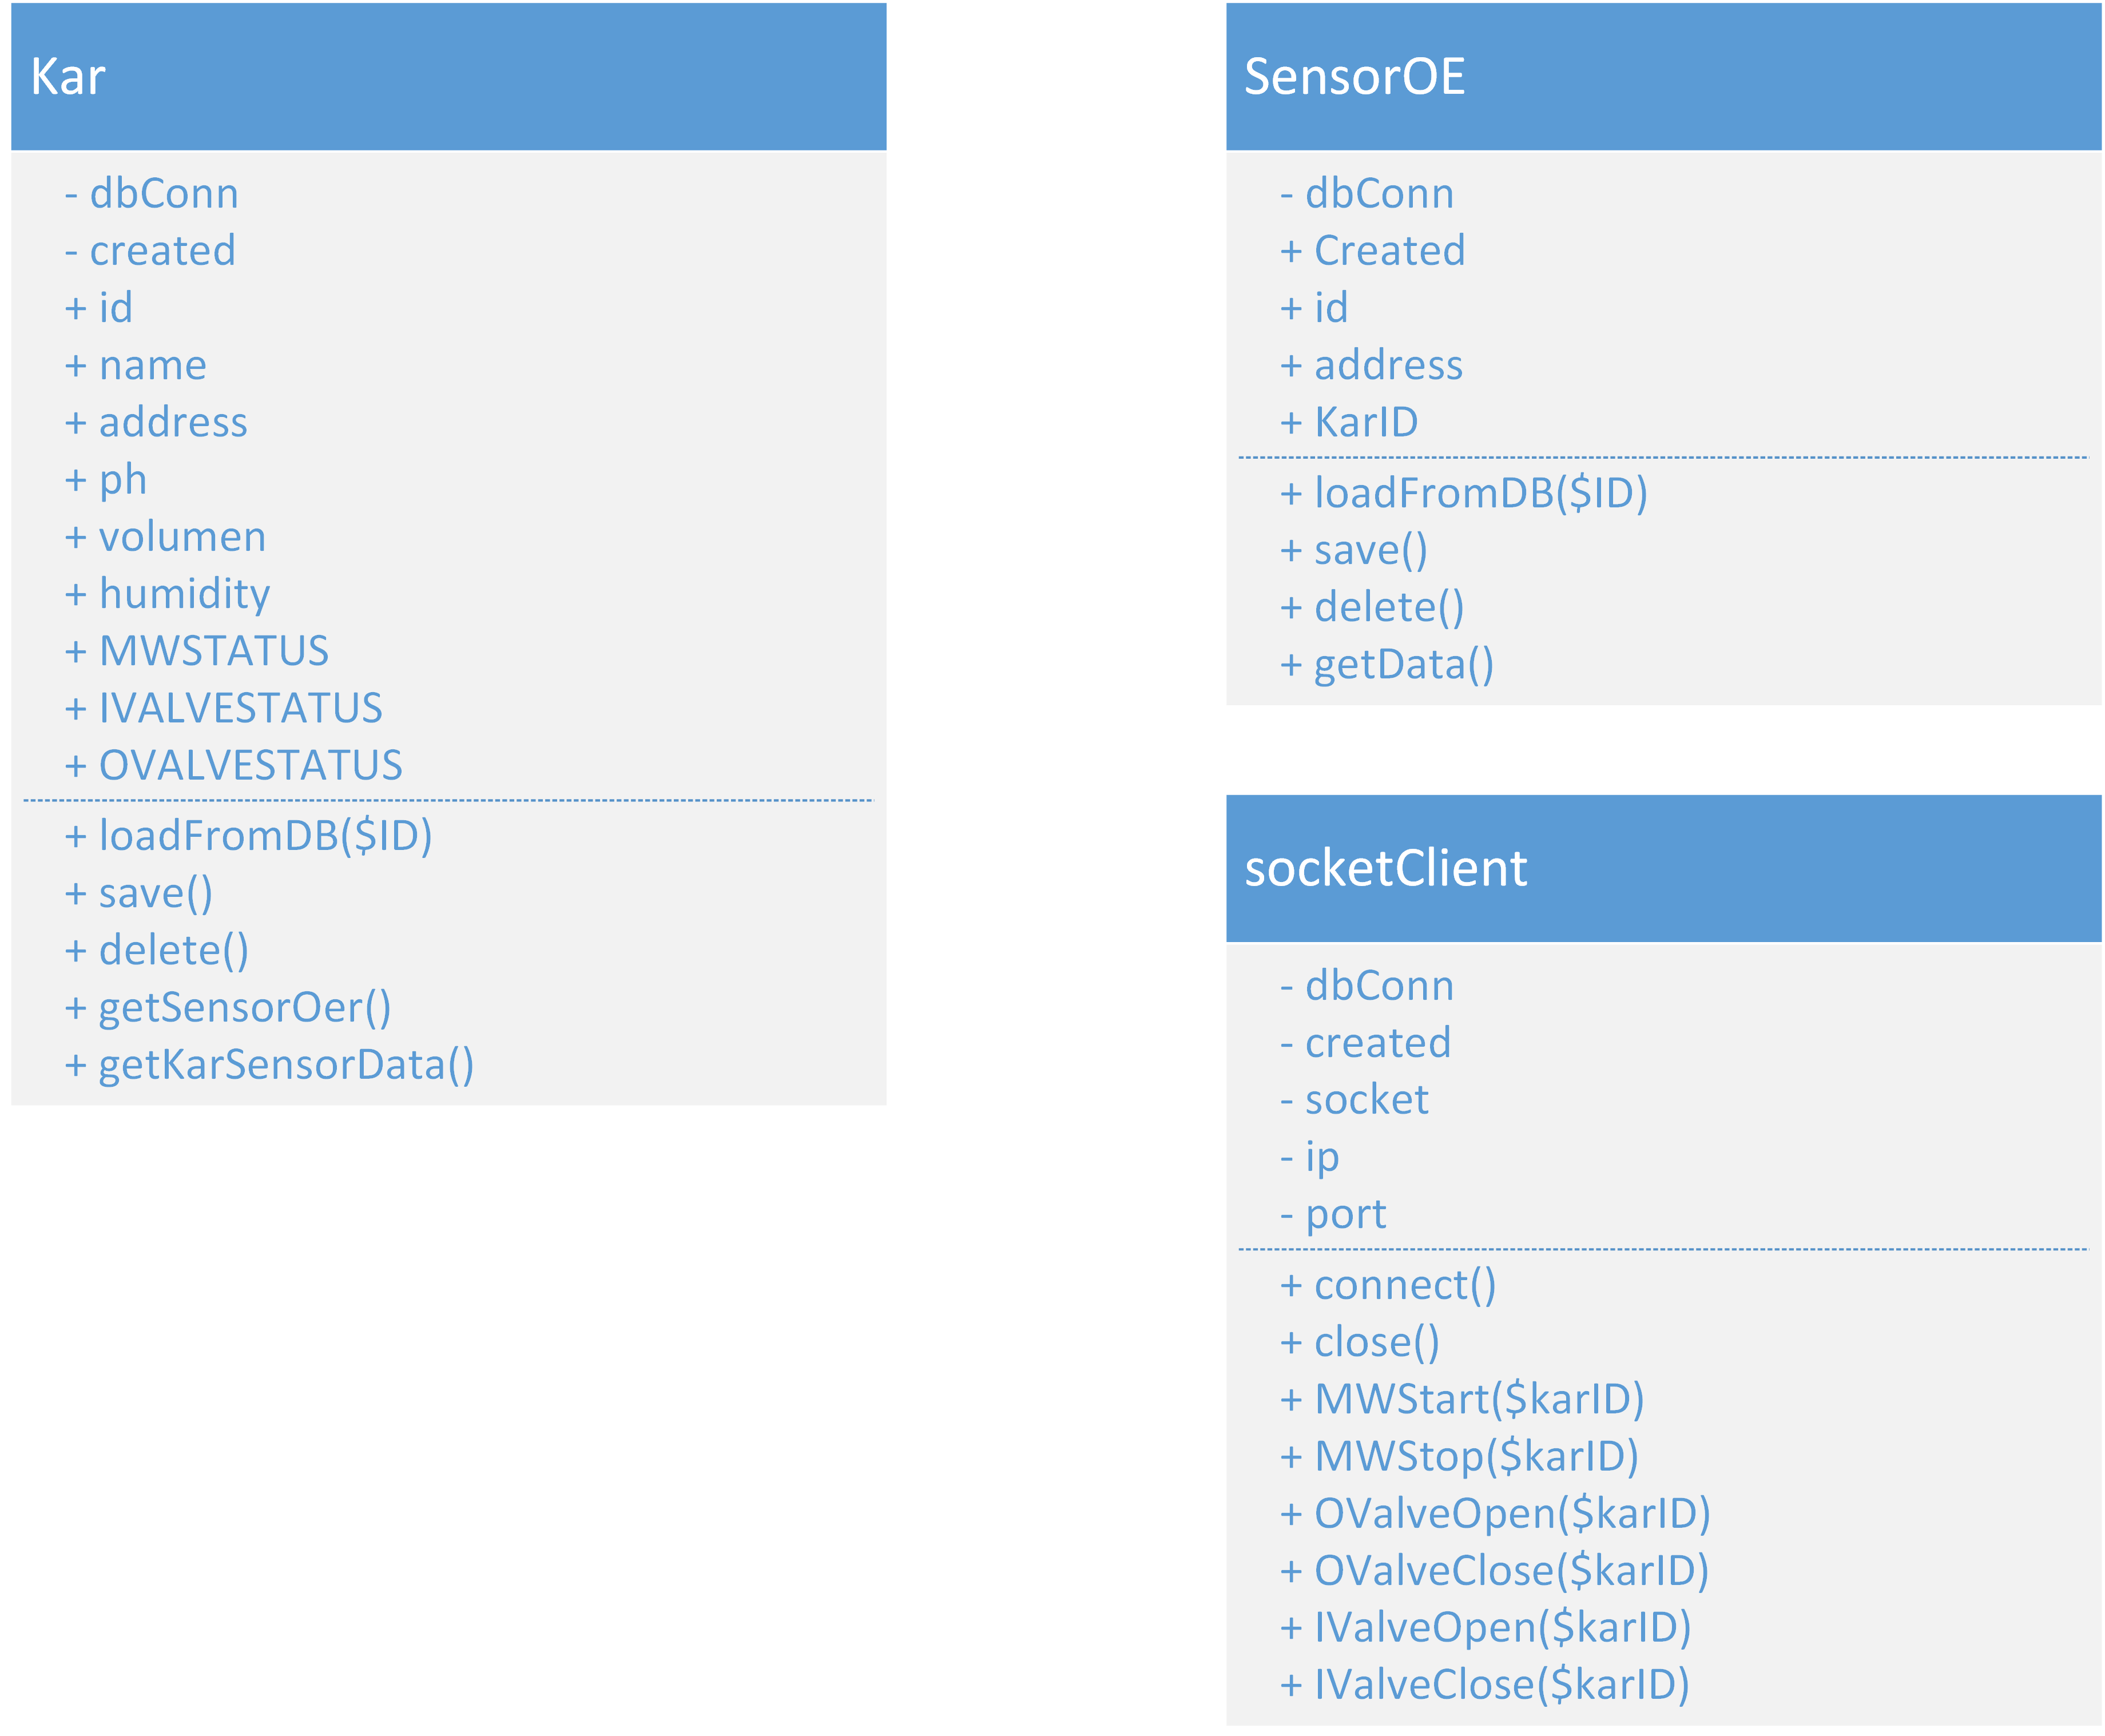
\includegraphics[width=0.7\textwidth]{SoftwareArkitektur/GUI/KlasseDiagram/photo/klasseDiagram_gui.PNG}
    \caption{Klassediagram for GUI}
    \label{fig:GUI_KD}
\end{figure}

Her kan man se der ikke er nogle forbindelse mellem de tre klasser, og det skyldes at de får alt deres information om de andre klasser gennem databasen.
 
\subsubsection{Kar klassen}
Kar klassen er en klasse, der giver mulighed for at tilgå et kar fra databasen og få alt dens information baseret på dens ID. Via klassens metoder kan de forskellige data i databasen blive redigeret, karet kan blive oprettet/slettet og man kan se hvilke \glslink{sensoroe}{Sensor Øer} der sider på karet. Den har følgende metoder:

\subsubsection{SensorOe klassen}
SensorOe klassen er en klasse, der giver mulighed for tilgå en Sensor Ø fra databasen og få alt dens information baseret på dens ID. Via klassens metoder kan de forskellige data i databasen blive redigeret, Sensor Øen kan blive oprettet/slettet og man kan se hvilket kar Sensir Øen tilhører. Den har følgende metoder:

\subsubsection{SocketClient klassen}
SocketClient klassen er en socket klient der anvendes til at sende beskeder direkte til FlexPMS, for at give besked om nogle ting systemet skal gøre. Den har følgende metoder: